%!TEX root = /Users/stevenmartell/Documents/CONSULTING/HumpbackChub/HBC_2011_Assessment/WRITEUP/HBCmain.tex

\section{Size Transition Matrix from Mark-Recapture data} % (fold)
\label{sec:size_transition_matrix_from_mark_recapture_data}


% Alternative method for constructing the Length Transition Matrix. (Move to Appendix?)
There is an alternative method for independently constructing annual length transition matrix based on individual capture-recapture information that incorporates both parametric uncertainty and measurement error.  The alternative method of constructing length-based transition matrices can be used as an alternative to internally estimating growth parameters, rather than jointly estimating them and introducing addition parameter confounding.  This method was recently described by \cite{hillary2010new}. In short, the method first estimates von Bertalanffy growth parameters based on the length-at-release and growth increment information, growth parameters are then sampled from the joint posterior distribution, and for each posterior sample measurement error is then added to the predicted growth increment  from $x_j$ to $x_{j'}$ and the overlap between $(x_{j'}-x^*) \cap (x_{j'}+x^*)$ is calculated.  To numerically approximate the length transition matrix, 1,000 samples from the joint posterior distribution are used to construct 1,000 length-transition matrixes ($P_{j,j'}$) and the mean values from the 1000 matrixes are used as the length transition matrix.

Growth parameters were estimated based on growth increment data from individual fish that were captured and recaptured in the subsequent year only.  Initially, growth increment data based on length-at-tagging and the most recent capture event was used (i.e., the longest time at liberty) were going to be used; but, upon further inspection of the raw data  there is evidence of changes in growth rates over time (see increasing negative slopes in Figure \ref{fig:FIGS_LSMR_fig:GrowthIncrements}).  To minimize the impact of changing growth rates, the growth increment data were based only on individuals that were captured and recaptured in the subsequent calendar year (Figure \ref{fig:FIGS_LSMR_fig:AnnualGrowthIncrements}), hereafter referred to as annual growth increment data.

\begin{figure}[htbp]
	\centering
		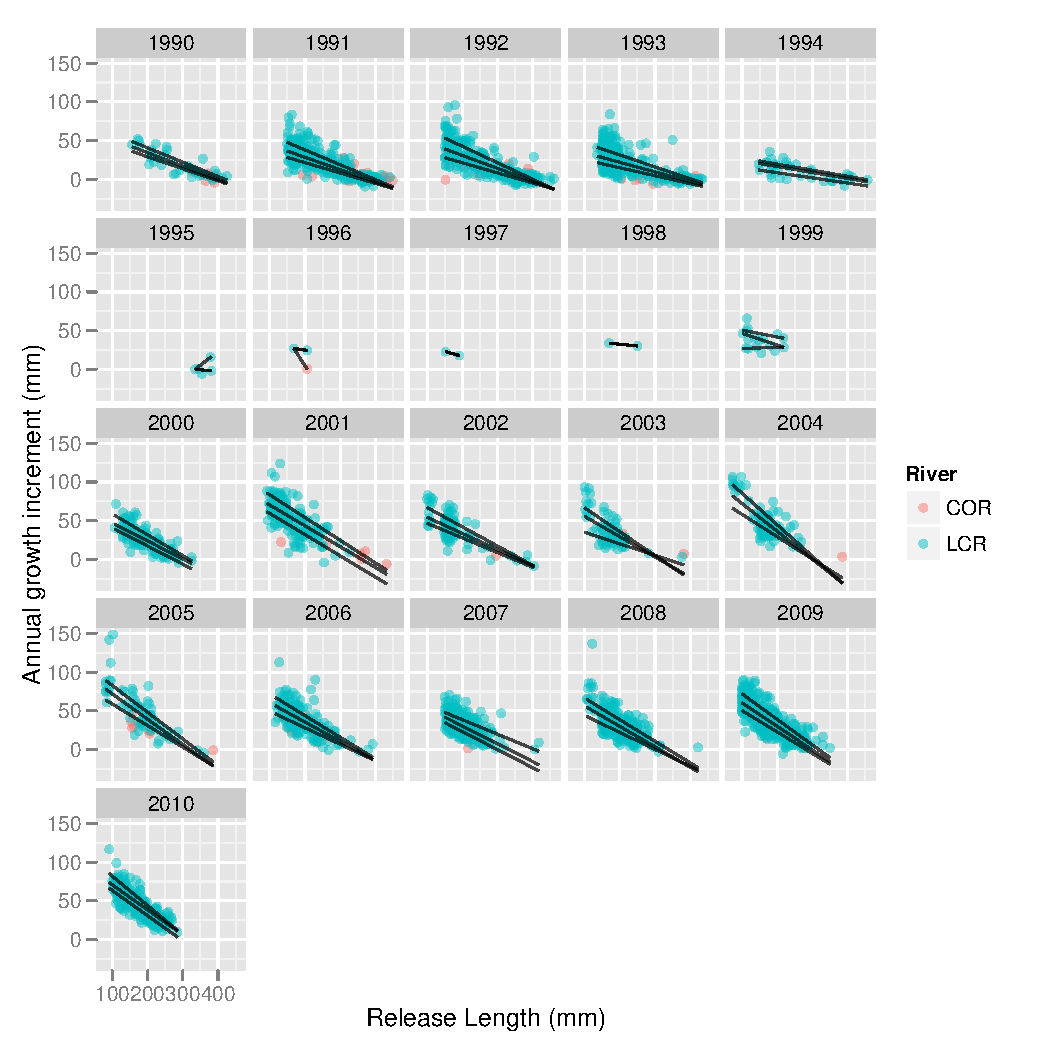
\includegraphics[width=6.5in]{../FIGS/LSMR/fig:GrowthIncrements.pdf}
	\caption{Growth increments by tag year for individually tagged humpback chub that have been at large for at least 1 year.   Recapture events could have occurred in either river. Fitted lines correspond to the 5, 50 and 95 percentiles of the data.}
	\label{fig:FIGS_LSMR_fig:GrowthIncrements}
\end{figure}

\begin{figure}[htbp]
	\centering
		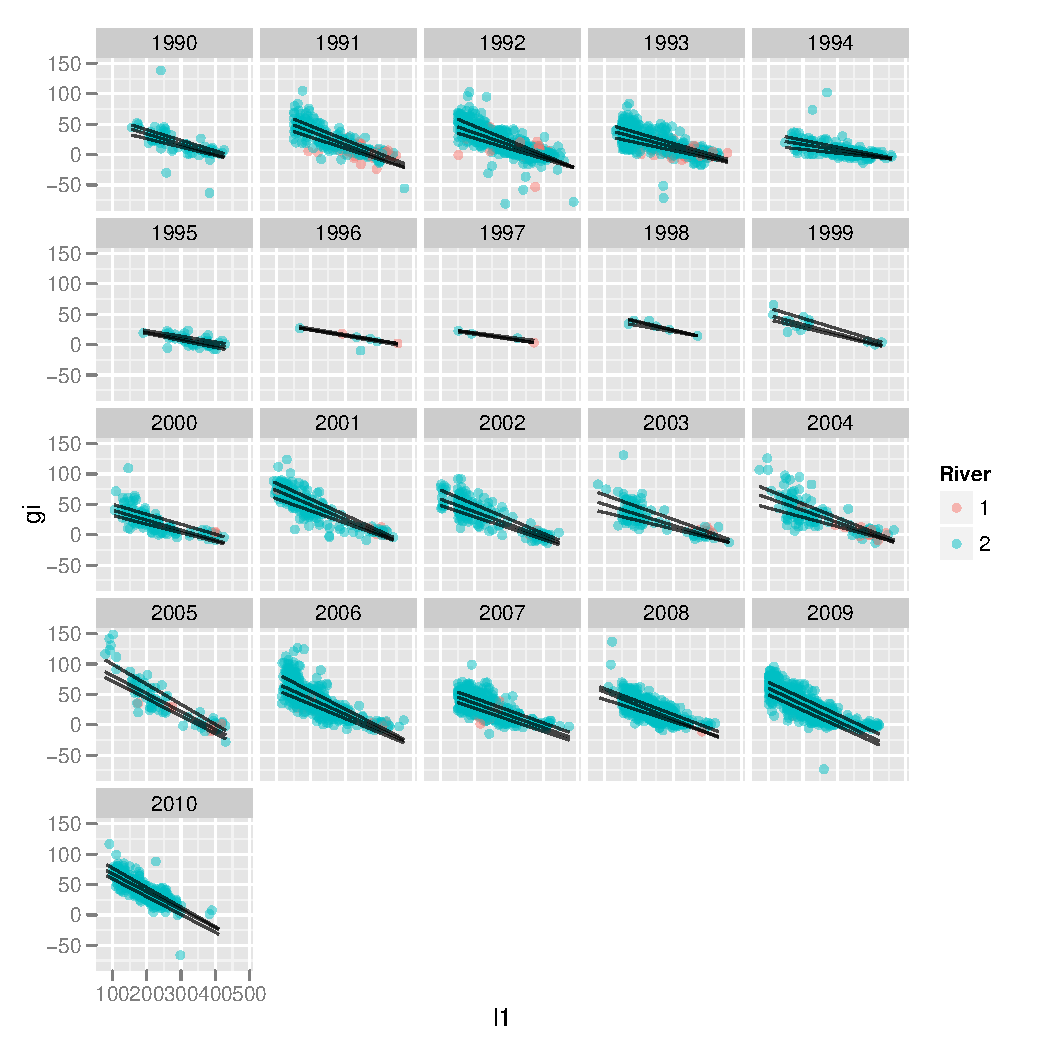
\includegraphics[width=6.5in]{../FIGS/LSMR/fig:AnnualGrowthIncrements.pdf}
	\caption{Annual growth increments of humpback chub of all fish captured and recaptured in the following year. River 2 corresponds to fish tagged in the Little Colorado River, River 1 the Colorado River. Fitted lines correspond to the 5, 50 and 95 percentiles of the data.}
	\label{fig:FIGS_LSMR_fig:AnnualGrowthIncrements}
\end{figure}


% section size_transition_matrix_from_mark_recapture_data (end)